\documentclass{article}
\usepackage{amsmath}
\usepackage{amssymb}
\usepackage{graphicx}
\usepackage{float}
\usepackage{enumitem}
\usepackage{forest}

\begin{document}

\title{Homework 3}
\author{Manyara Bonface Baraka - mbaraka}
\date{\today}
\maketitle

\section{Dimensionality of k-Nearest Neighbors (k-NN)}

 - Curse of Dimensionality: Is the phenomenon that is experienced when the number of
  dimensions or features in a dataset increases, and the volume of the space increases so fast that the available data becomes sparse.


%   Enumarate using alphabetically
\begin{enumerate}
  \item[a)] X is uniformly distributed on [0,1]. Predict the response at a test observation
  \textit{x} using the trainng observation that are within 10\% of the range of \textit{X} closest to \textit{x}.

  \subsubsection*{Solution}
  Defining interval for different cases.
  \begin{itemize}
        \item If $x$ is not too close to the edges that is $x \in [0.05, 0.95]$ then the interval is $[x-0.05, x+0.05]$
        \item From the example x = 0.6, then the interval is [0.55, 0.65]
        \[0.65 - 0.55 = 0.1\]

        \item If $x \le 0.05$ for instance 0.02, then the interval is $[0, 0.1]$
        \[0.1 - 0 = 0.1\]

        \item if $x \ge 0.95$ for instance 0.98, then the interval is $[0.9, 1]$
        \[1 - 0.9 = 0.1\]

        Therefore, since the range of X is 1: \textbf{the interval is 0.1}
  \end{itemize}

  \item[b)] When d = 2, we have $X_1$ and $X_2$ that are uniformly distributed on [0,1].
   Predict the response at a test observation \textit{x} using the training observation that
    is within 10\% of the range of \textit{X} closest to \textit{x}.

    \begin{itemize}
        \item Since the range for both the features is 0.1, this means:
        \[
        \text{Area of selection } = 0.1 \times 0.1 = 0.01
        \]

        \item Since they are uniformly distributed:
        \[1 \times 1 = 1\]

        \item Since the training points are uniformly distributed over the square therefore the 
        available observation is:
        \[
        \frac{\text{Area of selection}}{\text{Total area}} = \frac{0.01}{1} = 0.01 \quad \text{or 1\%}
        \]
  \end{itemize}

  \item [c)] When d = 100, we have $X_1, X_2, \ldots, X_{100}$ that are uniformly distributed on [0,1]. Each feature ranges in value from 0 to 1.
    Predict the response at a test observation \textit{x} using the training observation that is within 10\% of the range of \textit{X} closest to \textit{x}.
    What fraction of the available observations will we use to make the prediction?

    \begin{itemize}
        \item In d = 100, with the length of 0.1, the volume of the hypercube is:
        \[
        0.1^{100} = 10^{-100}   
        \]
    \end{itemize}


 \item[d)] Why does KNN struggle in high dimensions?
    \begin{itemize}
        \item The key observation from parts a-c is that:
         \begin{itemize}
            \item \textbf{For \textit{d = 1:}} The fraction of the available observations is 10\%, this is because the training points are close to the test points.
            \item \textbf{For \textit{d = 2:}} The fraction of the available observations is 1\%, we have fewer "nearby" points to rely on compared to d = 1.
            \item \textbf{For \textit{d = 100:}} The fraction of the available observations is $0.1^{100}$, this is a very small number. Almost no training points are close to the test point.
         \end{itemize}
        \item The reason this happens is due to the curse of Dimensionality:
         \begin{itemize}
            \item Neighborhood becomes sparser as the number of dimensions increases.
            \item The distance measures become less meaningful with the increase of dimension this is because
            in high dimensions the distance between any two points becomes almost the same.
            \item Since KNN relies on Neighborhood if there are not enough nearby training points, the prediction is unreliable.
         \end{itemize}
    \end{itemize}

 \item [e)] We wish to predict test observation by creating a d-Dimensionality hypercube centered around the test observation that contains an average of 10\% of the training observation
 For d = 1, 2, 100, what is the length of each side of the hypercube? How does the answer change as d increases, and what does it imply for the accuracy of the k-nearest neighbors when d is large?\\

 \begin{itemize}
    \item If we need to contain 10\% of all observations the volume should be 0.1
    \item For d-Dimensionalityal hypercube:
    \[
    \text{volume} = (\text{Side length})^d = 0.1
    \]
    let the side length be $s$:
    \[
    s^d = 0.1 
    \]
   \[s = 0.1^{1/d}\]
    
    \item Finding the side length for:
    \begin{itemize}
        \item \textbf{For d = 1:} $s = 0.1^{1/1} = 0.1$
        \item \textbf{For d = 2:} $s = 0.1^{1/2} = 0.316$
        \item \textbf{For d = 100:} $s = 0.1^{1/100} = 0.977$
    \end{itemize}

    \item As d increases the side length approaches 1, this indicates that the hypercube needs to grow in size to include 10\% of the training data.
    \item For large d, the hypercube will be very large and will contain almost all the training data. This implies that the KNN will be less reliable as the number of dimensions increases.
    \item The accuracy of the KNN will decrease as the number of dimensions increases.

    
 \end{itemize}


\end{enumerate}

\clearpage

\section{Decision Trees}
\begin{itemize}
   \item Entropy is use to measure the impurity of a node in a decision tree.
   \item It helps us in to measure the uncertainty or randomness in a dataset. We use entropy for:
     \begin{itemize}
      \item Decide whiche feature to split (higher reduction in entropy its a better split)
      \item Evaluate how mixed/uncertain the dataset is (lower entropy leads to pure groups) 
     \end{itemize}
   \item Entropy is defined as:
   \[
   H(S) = -\sum_{i=1}^{c} p_i \log_2 p_if
   \]
   where $p_i$ is the probability of class i in the dataset.
   \item High entropy means the dataset is mixed, while low entropy means the dataset is pure.
   \item Information Gain is the measure of the reduction in entropy after the dataset is split on an attribute.
   \item Information Gain is defined as:
   \[\text{IG = Entropy(before split) - Entropy(after split)}\]
   % \[
   % IG(S, A) = H(S) - \sum_{v \in Values(A)} \frac{|S_v|}{|S|} H(S_v)
   % \]
   % where $S_v$ is the subset of the dataset for a given value of attribute A.
\end{itemize}

\begin{enumerate}[label=\alph*)]
   \item What is the entropy of Phone Usage? (Calculate the entropy in log\_2 base and round to 4 decimal places)
   \subsubsection*{Solution}
   \begin{itemize}
      \item Count occurances:
      \begin{itemize}
         \item Low: 7
         \item Medium: 5
         \item High: 3
         \item Total Count: 15
      \end{itemize}

      \item Calculate the Entropy of phone Usage:
      \[
      \text{H(Phone Usage ) = -(p\_low * log2(p\_low) + p\_medium * log2(p\_medium) + p\_high * log2(p\_high))}
      \]

      where:
      \begin{itemize}
         \item $p_{low} = \frac{7}{15}$
         \item $p_{medium} = \frac{5}{15}$
         \item $p_{high} = \frac{3}{15}$
      \end{itemize}

      Substute:
      \[
      = -(\frac{7}{15} \log_2(\frac{7}{15}) + \frac{5}{15} \log_2(\frac{5}{15}) + \frac{3}{15} \log_2(\frac{3}{15}))
      \]
      \[
      \approx 1.5058
      \]
   
   \end{itemize}

   \item Find the information gain {IG} from each features (relationship status, age, eductaion levarianceel and income). Which features
   should be choosen as the root of th tree? Show calculations for the IG and explain the choise in a sentence. (Calculate entropy in log\_2 base and round to 4 decimal places) 
   \begin{itemize}
      \item Information gain measures how much the entropy is reduced when splitting the dataset.
      \item Calculated by:
      \[
      \text{IG(Feature (Y)) = H(Phone Usage) - H(Phone Usage | Feature (Y))}
      \]
   \end{itemize}
   \subsubsection*{Solution}
   \begin{itemize}
      \item \textbf{relationship status:}
      \begin{itemize}
         \item Count of relationship status:
         \begin{itemize}
            \item Single: 5 Low, 0 Medium, 0 High \textbf{(5)}
            \item Married: 0 Low, 1 Medium, 3 High \textbf{(4)}
            \item In a relationship: 2 Low, 4 Medium,  0 High \textbf{(6)}
         \end{itemize}
         \item Calculate the conditional entropy for each relationship status:
         \begin{itemize}
            \item Single:
            \[
            H(Phone Usage | Single) = -(\frac{5}{5} \log_2(\frac{5}{5}) + \frac{0}{5} \log_2(\frac{0}{5}) + \frac{0}{5} \log_2(\frac{0}{5}))
            \]
            \[
            = 0
            \]
            \item Married:
            \[
            H(Phone Usage | Married) = -(\frac{0}{4} \log_2(\frac{0}{4}) + \frac{1}{4} \log_2(\frac{1}{4}) + \frac{3}{4} \log_2(\frac{3}{4}))
            \]
            \[
            \approx 0.8113
            \]
            \item In a relationship:
            \[
            H(Phone Usage | In a relationship) = -(\frac{2}{6} \log_2(\frac{2}{6}) + \frac{4}{6} \log_2(\frac{4}{6}) + \frac{0}{6} \log_2(\frac{0}{6}))
            \]
            \[
            \approx 0.9183
            \]
      \end{itemize}
      \item Calculate the weighted average of the conditional entropy:
      \[
      H(Phone Usage | Relationship Status) = \frac{5}{15} \times 0 + \frac{4}{15} \times 0.8113 + \frac{6}{15} \times 0.9183
      \]
      \[
      \approx 0.5836
      \]

      \item Calculate the Information Gain:
      \[
      IG(Relationship Status) = 1.5058 - 0.5836
      \]
      \[
      \approx 0.9222
      \]
\end{itemize}

\item \textbf{Age:}
\begin{itemize}
   \item Count of Age:
   \begin{itemize}
      \item \(\ge\) 25: 6 Low, 1 Medium, 2 High \textbf{(9)}
      \item \(\leq\) 25: 1 Low, 4 Medium, 1 High \textbf{(6)}
   \end{itemize}
   \item Calculate the conditional entropy for each age:
   \begin{itemize}
      \item \(\ge\) 25:
      \[
      H(Phone Usage | \ge 25) = -(\frac{6}{9} \log_2(\frac{6}{9}) + \frac{2}{9} \log_2(\frac{2}{9}) + \frac{1}{9} \log_2(\frac{1}{9}))
      \]
      \[
      \approx 1.2244
      \]
      \item \(\leq\) 25:
      \[
      H(Phone Usage | \leq 25) = -(\frac{1}{6} \log_2(\frac{1}{6}) + \frac{1}{6} \log_2(\frac{1}{6}) + \frac{4}{6} \log_2(\frac{4}{6}))
      \]
      \[
      \approx 1.2516
      \]
   \end{itemize}
   \item Calculate the weighted average of the conditional entropy:
   \[
   H(Phone Usage | Age) = \frac{9}{15} \times 1.2244 + \frac{6}{15} \times 1.2516
   \]
   \[
   \approx 1.2350
   \]
   \item Calculate the Information Gain:
   \[
   IG(Age) = 1.5058 - 1.2350
   \]
   \[
   \approx 0.2708
   \]
\end{itemize}

\item \textbf{Education Level:}
\begin{itemize}
   \item Count of Education Level:
   \begin{itemize}
      \item High School: 4 Low, 0 Medium, 0 High \textbf{(4)}
      \item College: 0 Low, 5 Medium, 0 High \textbf{(5)}
      \item University: 3 Low, 0 Medium,3 High \textbf{(6)}
   \end{itemize}
   \item Calculate the conditional entropy for each education level:
   \begin{itemize}
      \item High School:
      \[
      H(Phone Usage | High School) = -(\frac{4}{4} \log_2(\frac{4}{4}) + \frac{0}{4} \log_2(\frac{0}{4}) + \frac{0}{4} \log_2(\frac{0}{4}))
      \]
      \[
      = 0
      \]
      \item College:
      \[
      H(Phone Usage | College) = -(\frac{0}{5} \log_2(\frac{0}{5}) + \frac{5}{5} \log_2(\frac{5}{5}) + \frac{0}{5} \log_2(\frac{0}{5}))
      \]
      \[
      = 0
      \]
      \item University:
      \[
      H(Phone Usage | University) = -(\frac{3}{6} \log_2(\frac{3}{6}) + \frac{0}{6} \log_2(\frac{0}{6}) + \frac{3}{6} \log_2(\frac{3}{6}))
      \]
      \[
      \approx 1
      \]
   \end{itemize}
   \item Calculate the weighted average of the conditional entropy:
   \[
   H(Phone Usage | Education Level) = \frac{4}{15} \times 0 + \frac{5}{15} \times 0 + \frac{6}{15} \times 1
   \]
   \[
   \approx 0.4
   \]
   \item Calculate the Information Gain:
   \[
   IG(Education Level) = 1.5058 - 0.4
   \]
   \[
   \approx 1.1058
   \]

\end{itemize}
\item \textbf{Income:}
\begin{itemize}
   \item Count of Income:
   \begin{itemize}
      \item \(\leq \) 50K: 3 Low, 2 Medium, 3 High \textbf{(8)}
      \item \(\ge\) 50K: 4 Low, 3 Medium, 0 High \textbf{(7)}
\end{itemize}
\item Calculate the conditional entropy for each income:
\begin{itemize}
   \item \(\leq \) 50K:
   \[
   H(Phone Usage | \leq 50K) = -(\frac{3}{8} \log_2(\frac{3}{8}) + \frac{2}{8} \log_2(\frac{2}{8}) + \frac{3}{8} \log_2(\frac{3}{8}))
   \]
   \[
   \approx 1.5613
   \]
   \item \(\ge\) 50K:
   \[
   H(Phone Usage | \ge 50K) = -(\frac{4}{7} \log_2(\frac{4}{7}) + \frac{3}{7} \log_2(\frac{3}{7}) + \frac{0}{7} \log_2(\frac{0}{7}))
   \]
   \[
   \approx 0.9852
   \]
\end{itemize}
\item Calculate the weighted average of the conditional entropy:
\[
H(Phone Usage | Income) = \frac{8}{15} \times 1.5613 + \frac{7}{15} \times 0.9852
\]
\[
\approx 1.2925
\]
\item Calculate the Information Gain:
\[
IG(Income) = 1.5058 - 1.2925
\]
\[
\approx 0.2133
\]
\end{itemize}


\textbf{The features choice for Root Node:} The feature with the highest information gan is \textbf(Education)
 with IG \(\approx 1.1058\). This feature will be chosen as the root of the tree because 
 it provides the highest reduction in entropy when splitting the dataset.

\end{itemize}

\item Using the root node you have choosen determine the rest of the nodes in the decision tree for the abovariancee data.
Draw the full decision tre i.e keep splittng the nodes untill further splits do not lead to any information gain (you may not
need all the features for this). For each split, show your working on why you chose this feature based on information gain.
\subsubsection*{Solution}
\begin{itemize}
   \item Since we have chosen Education as the root node, we will split the dataset based on the values of Education.
   \item We will calculate the Information Gain for each feature at each node and choose the feature with the highest Information Gain.
   \item We will continue splitting the nodes until further splits do not lead to any Information Gain.
   \item The decision tree will look like this:
   \item \textbf{Root Node: Education}
   \begin{itemize}
      \item \textbf{Branch1:High School}
      \begin{itemize}
         \item Count of Phone Usage:
         \begin{itemize}
            \item Low: 4
            \item Medium: 0
            \item High: 0
         \end{itemize}
         \item Since all the Phone Usage values are Low, this node is pure and we do not need to split further.
      \end{itemize}
      \item \textbf{Branch2: College}
      \begin{itemize}
         \item Count of Phone Usage:
         \begin{itemize}
            \item Low: 0
            \item Medium: 5
            \item High: 0
         \end{itemize}
         \item Since all the Phone Usage values are Medium, this node is pure and we do not need to split further.
         \end{itemize}
      \item \textbf{Branch3: University}
      \begin{itemize}
         \item Count of Phone Usage:
         \begin{itemize}
            \item Low: 3
            \item Medium: 0
            \item High: 3
         \end{itemize}
         \item The branch is impure,we need to split it further.
         \item To considet the next split, from the information gain we have for each features within university:
         \begin{itemize}
            \item \textbf{Relationship Status:} = 0.9222
            \item \textbf{Age:} = 0.2708
            \item \textbf{Income:} = 0.2133
         \end{itemize}
         \item The feature with the highest Information Gain is \textbf{Relationship Status}.
      \end{itemize}
   \end{itemize}
   \item \textbf{Splitting on Relationship status within University}
   \begin{itemize}
      \item \textbf{Branch1: Single}
      \begin{itemize}
         \item Count of Phone Usage:
         \begin{itemize}
            \item Low: 5
            \item Medium: 0
            \item High: 0
         \end{itemize}
         \item Since all the Phone Usage values are Low, this node is pure and we do not need to split further.
      \end{itemize}
      \item \textbf{Branch2: In a relationship}
      \begin{itemize}
         \item Count of Phone Usage:
         \begin{itemize}
            \item Low: 2
            \item Medium: 4
            \item High: 0
         \end{itemize}
         \item Since all the Phone Usage values are Medium, this node is pure and we do not need to split further.
      \end{itemize}
      \item \textbf{Branch3: Married}
      \begin{itemize}
         \item Count of Phone Usage:
         \begin{itemize}
            \item Low: 0
            \item Medium: 1
            \item High: 3
         \end{itemize}
         \item The branch is impure, we need to split it further.
         \item To consider the next split, from the information gain we have for each features within Married:
         \begin{itemize}
            \item \textbf{Age:} = 0.9183
            \item \textbf{Income:} = 0.8113
         \end{itemize}
         \item The feature with the highest Information Gain is \textbf{Age}.
      \end{itemize}
   \end{itemize}
   \item The tree will be:\\
   \begin{forest}
      [Education
         [High School
            [Low]
         ]
         [College
            [Medium]
         ]
         [University
            [Relationship Status
               [Single
                  [Low]
               ]
               [In a relationship
                  [Medium]
               ]
               [Married
                  [Age
                     [\(\ge 25\)
                        [Low]
                     ]
                     [\(\le 25\)
                        [Medium]
                     ]
                  ]
               ]
            ]
         ]
      ]
   \end{forest}
\end{itemize}
\end{enumerate}

\clearpage

\section{Random Forest}
\begin{enumerate}[label=\alph*)]
   \item Build 3 decision trees using two features out of the three of each tree. Use the information gain to decide the feature to split on .Use majoity
   voting if all the samples in a leaf node do not have the same label.

   \subsubsection*{Solution}
   \begin{itemize}
      \item \textbf{Entropy of the Getting Sick}
      \begin{itemize}
         \item Count of Getting Sick:
         \begin{itemize}
            \item Yes: 4
            \item No: 4
         \end{itemize}
         \item Calculate the Entropy of Getting Sick:
         \[
         H(Getting Sick) = -(\frac{4}{8} \log_2(\frac{4}{8}) + \frac{4}{8} \log_2(\frac{4}{8}))
         \]
         \[
         = 1
         \]
      \end{itemize}
      \item \textbf{Information Gain for each feature:}
      \begin{itemize}
         \item \textbf{Age(A):}
         \begin{itemize}
            \item Count of Age:
            \begin{itemize}
               \item \textbf{Old} 3 yes, 3 no
               \item \textbf{Young} 1 yes, 1 no
            \end{itemize}
            \item Calculate the conditional entropy for each age:
            \begin{itemize}
               \item \textbf{Old:}
               \[
               H(Getting Sick | Old) = -(\frac{3}{6} \log_2(\frac{3}{6}) + \frac{3}{6} \log_2(\frac{3}{6}))
               \]
               \[
               = 1
               \]
               \item \textbf{Young:}
               \[
               H(Getting Sick | Young) = -(\frac{1}{2} \log_2(\frac{1}{2}) + \frac{1}{2} \log_2(\frac{1}{2}))
               \]
               \[
               = 1
               \]
            \end{itemize}
            \item Calculate the weighted average of the conditional entropy:
            \[
            H(Getting Sick | Age) = \frac{6}{8} \times 1 + \frac{2}{8} \times 1
            \]
            \[
            = 1
            \]
            \item Calculate the Information Gain:
            \[
            IG(Age) = 1 - 1
            \]
            \[
            = 0
            \]
         \end{itemize}
         \item \textbf{Social Distance(S):}
         \begin{itemize}
            \item Count of Social Distance:
            \begin{itemize}
               \item \textbf{Yes} 0 yes, 4 no
               \item \textbf{No} 4 yes, 0 no
            \end{itemize}
            \item Calculate the conditional entropy for each social distance:
            \begin{itemize}
               \item \textbf{Yes:}
               \[
               H(Getting Sick | Yes) = -(\frac{0}{4} \log_2(\frac{0}{4}) + \frac{4}{4} \log_2(\frac{4}{4}))
               \]
               \[
               = 0
               \]
               \item \textbf{No:}
               \[
               H(Getting Sick | No) = -(\frac{4}{4} \log_2(\frac{4}{4}) + \frac{0}{4} \log_2(\frac{0}{4}))
               \]
               \[
               = 0
               \]
            \end{itemize}
            \item Calculate the weighted average of the conditional entropy:
            \[
            H(Getting Sick | Social Distance) = \frac{4}{8} \times 0 + \frac{4}{8} \times 0
            \]
            \[
            = 0
            \]
            \item Calculate the Information Gain:
            \[
            IG(Social Distance) = 1 - 0
            \]
            \[
            = 1
            \]
         \end{itemize}
         \item \textbf{Handwashing (H):}
         \begin{itemize}
            \item Count of Handwashing:
            \begin{itemize}
               \item \textbf{Yes} 1 yes, 3 no
               \item \textbf{No} 3 yes, 1 no
            \end{itemize}
            \item Calculate the conditional entropy for each handwashing:
            \begin{itemize}
               \item \textbf{Yes:}
               \[
               H(Getting Sick | Yes) = -(\frac{1}{4} \log_2(\frac{1}{4}) + \frac{3}{4} \log_2(\frac{3}{4}))
               \]
               \[
               \approx 0.8113
               \]
               \item \textbf{No:}
               \[
               H(Getting Sick | No) = -(\frac{3}{4} \log_2(\frac{3}{4}) + \frac{1}{4} \log_2(\frac{1}{4}))
               \]
               \[
               \approx 0.8113
               \]      
            \end{itemize}
            \item Calculate the weighted average of the conditional entropy:
            \[
            H(Getting Sick | Handwashing) = \frac{4}{8} \times 0.8113 + \frac{4}{8} \times 0.8113
            \]
            \[
            \approx 0.8113
            \]
            \item Calculate the Information Gain:
            \[
            IG(Handwashing) = 1 - 0.8113
            \]
            \[
            \approx 0.1887
            \]
         \end{itemize}
      \end{itemize}
      \item \textbf{Tree 1: Social Distance (1) and Handwashing(0.8113)}
      \begin{itemize}
         \item The feature with the highest Information Gain is \textbf{Social Distance}.
         \item The tree will be:\\
         
         \begin{forest}
            [Social Distance
               [Yes
                  [No]
               ]
               [No
                  [Yes]
               ]
            ]
         \end{forest}
      \end{itemize}
      \item \textbf{Tree 2: Age(0) and Social Distance(1)}
      \begin{itemize}
         \item The feature with the highest Information Gain is \textbf{Social Distance}.
         \item The tree will be:\\
         
         \begin{forest}
            [Social Distance
               [Yes
                  [No]
               ]
               [No
                  [Yes]
               ]
            ]
         \end{forest}
      \end{itemize}
      \item \textbf{Tree 3: Age(0) and Handwashing(0.8113)}
      \begin{itemize}
         \item The feature with the highest Information Gain is \textbf{Handwashing}.
         \item The tree will be:\\
         
         \begin{forest}
            [Handwashing
               [Yes
                  [No]
               ]
               [No
                  [Yes]
               ]
            ]
         \end{forest}
      \end{itemize}
   \end{itemize}  

   \item Given a new data point with the reatures (A = old, S=yes, H = no), use the trees you  learned from part (a) to predict whether this person is sick.
   \subsubsection*{Solution}
   \begin{itemize}
      \item \textbf{Using Tree 1: Social Distance and Handwashing}\\
      \begin{itemize}
         \item The new data point has the features: Social Distance = Yes, Handwashing = No.
         \item The tree will predict that the person is \textbf{No}.
      \end{itemize}
      \item \textbf{Using Tree 2: Age and Social Distance}\\
      \begin{itemize}
         \item The new data point has the features: Social Distance = Yes.
         \item The tree will predict that the person is \textbf{No}.
      \end{itemize}
      \item \textbf{Using Tree 3: Age and Handwashing}\\
      \begin{itemize}
         \item The new data point has the features: Handwashing = No.
         \item The tree will predict that the person is \textbf{Yes}.
      \end{itemize}
   \end{itemize}
   Final prediction using majoity voting will be: \textbf{No}

   \item Briefly in 1-2 sentences comment on the advantage of random forests over decision tress from the perspective of bias-variance tradeoff.
   \subsubsection*{Solution}
   - Random forest are better than decision trees in terms of bias-variance tradeoff because they reduce
   overfitting and improve the model generalization. They generally reduce variance by averaging multiple decision trees that is through
   ensemble learning, this improves the overal performance of the model.
\end{enumerate}

\clearpage

\section{Adaboost}
- Unlike random forest, Adaboost is an ensemble method that works by combining multiple weak learners to create a strong learner.\\
- Adaboost works by assigning weights to each training example and adjusting the weights of the incorrectly classified dataset.\\
Consider the training dataset with N = 10 points and 2-D featuress x = (x1, x2) as shown in the figure above. In this problem we will use binary
linear decision boundary as the base classier and perfom two iterations of Adaboost.\\
\begin{enumerate}[label=\alph*)]
   \item Starting with equal weights \(w\_1(n) = 1/10\) for all \(N = 10\) points, which of the decision boundaries shown below gives the lowest error \(\epsilon\_1\)?
   Select one of the answers:
   \begin{itemize}
      \item Predict \(y = 1\) if \(x2 \leq 0.5\)
      \item Predict \(y = 1\) if \(-x1 + x2 \leq -0.5\)
      \item Predict \(y = 1\) if \(-x1 + x2 \leq 0.5\)
   \end{itemize}
   \begin{figure}[H]
      \centering
      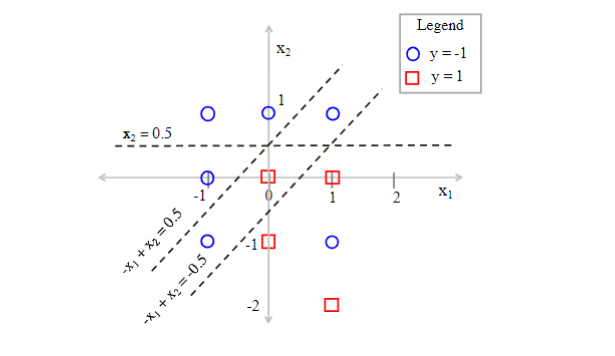
\includegraphics[width=1\linewidth]{image.png}
  \end{figure}
   \subsubsection*{Solution}
   \begin{itemize}
      \item Option 1: correct missclassification{error} = 3/10 = 0.3
      \item Option 2: correct missclassification{error} = 2/10 = 0.2
      \item Option 3: correct missclassification{error} = 3/10 = 0.3
   \end{itemize}
   The decision boundary that gives the lowest error is \textbf{Predict \(y = 1\) if \(-x1 + x2 \leq -0.5\)} - 
   \textbf{b}

   \item Compute the error \(\epsilon_1\) and the contribution \(\beta\_1\) of the dicision boundary chosen in part (a) above.\\
   \subsubsection*{Solution}
   \begin{itemize}
      \item The error is given by:
      \[
      \epsilon_1 = \sum_{i=1}^{N} w_1(i) \times \text{missclassification error}
      \]
      \[
      = \frac{1}{10} \times 2 = 0.2
      \]
      \item The contribution is given by:
      \[
      \beta_1 = \frac{1}{2} \log_2(\frac{1 - \epsilon_1}{\epsilon_1})
      \]
      \[
      = \frac{1}{2} \log_2(\frac{1 - 0.2}{0.2})
      \]
      \[
      \approx 1
      \]
   \end{itemize}

   \item  Compute the updated and normalized weights \(w_2(n)\) for each of the data points as follows.\\
   \begin{figure}[H]
      \centering
      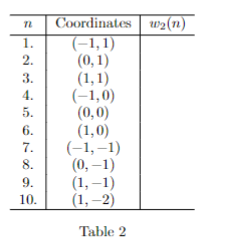
\includegraphics[width=0.5\linewidth]{image1.png}
  \end{figure}
   \subsubsection*{Solution}
   The formular for updating weights is:
   \[
      w_{t+1}(n) \propto w_t(n) \cdot 2^{-\beta_t y_n h_t(x_n)}
   \]
   where:
   \begin{itemize}
      \item \(w\_t(n)\) is the weight of sample n at iteration t.
      \item \(beta_t\) the weight of weak classifier = 1
      \item \(y\_n\) true label of the samples (1 or -1)
      \item \(h_t(x_n)\) prediction of the weak classifier for the sample.
   \end{itemize}
   \begin{itemize}
      \item Calculating the unnormalised weights:
      \begin{itemize}
         \item For correctly classified points(where \(y_n = h_t(x_n)\))
         \[
         w_2(n) = w_1(n) \times 2^{-1} = \frac{1}{10} \times \frac{1}{2} = \frac{1}{20}
         \]
          \item For misclassified points (where \(y_n \neq h_t(x_n)\))
          \[ 
          w_2(n) = w_1(n) \times 2^{1} = \frac{1}{10} \times 2 = \frac{2}{10} = \frac{1}{5}
          \]
      \end{itemize}
      \item identify correct and incorrectly classifications using the chosen weak classifier from part (a) \(y = 1\) if \(-x_1 + x_2 \le -0.5\)
      \begin{table}[h!]
         \centering
         \begin{tabular}{|c|c|c|c|c|c|}
         \hline
         Index & Coordinates $(x_1, x_2)$ & True Label $y_n$ & Classifier Prediction $h_1(x_n)$ & Correct? & Weight Update \\
         \hline
         1 & $(-1, 1)$ & -1 & -1 & correct & \(\frac{1}{20}\) \\
         \hline
         2 & $(0, 1)$ & -1 & -1 & correct & \(\frac{1}{20}\) \\
         \hline
         3 & $(1, 1)$ & -1 & -1 & correct & \(\frac{1}{20}\) \\
         \hline
         4 & $(-1, 0)$ & -1 & -1 & correct & \(\frac{1}{20}\) \\
         \hline
         5 & $(0, 0)$ & 1 & -1 & incorrect & \(\frac{1}{5}\) \\
         \hline
         6 & $(1, 0)$ & 1 & 1 & correct & \(\frac{1}{20}\) \\
         \hline
         7 & $(-1, -1)$ & -1 & -1 & correct & \(\frac{1}{20}\) \\
         \hline
         8 & $(0, -1)$ & 1 & 1 & correct & \(\frac{1}{20}\) \\
         \hline
         9 & $(1, -1)$ & -1 & 1 & incorrect & \(\frac{1}{5}\) \\
         \hline
         10 & $(1, -2)$ & 1 & 1 & correct & \(\frac{1}{20}\) \\
         \hline
         \end{tabular}
         % \caption{Table Representation with Coordinates, Labels, Predictions, and Weight Updates}
         \end{table}
         \item Normalizing the weights \(w_2(n)\):
         \[
         \sum_{i=1}^{N} w_2(i) = \frac{1}{20} \times 8 + \frac{1}{5} \times 2 = \frac{8}{20} + \frac{4}{20} = \frac{12}{20} = \frac{4}{5}
         \]
         \[
         w_2(n) = \frac{w_2(n)}{\sum_{i=1}^{N} w_2(i)}
         \]
         \begin{itemize}
            \item For correctly classified points:
            \[
            w_2(n) = \frac{\frac{1}{20}}{\frac{4}{5}} = \frac{1}{20} \times \frac{5}{4} = \frac{1}{16}
            \]
            \item For misclassified points:
            \[
            w_2(n) = \frac{\frac{1}{5}}{\frac{4}{5}} = \frac{1}{5} \times \frac{5}{4} = \frac{1}{4}
            \]
         \end{itemize}
      \item Finalized normalized weights \(w_2(n)\) table with index cordinates and the normalized new weights \(w_2(n)\).
      \begin{table}[h!]
         \centering
         \begin{tabular}{|c|c|c|}
         \hline
         Index & Coordinates $(x_1, x_2)$ & Normalized Weight $w_2(n)$ \\
         \hline
         1 & $(-1, 1)$ & \(\frac{1}{16}\) \\
         \hline
         2 & $(0, 1)$ & \(\frac{1}{16}\) \\
         \hline
         3 & $(1, 1)$ & \(\frac{1}{16}\) \\
         \hline
         4 & $(-1, 0)$ & \(\frac{1}{16}\) \\
         \hline
         5 & $(0, 0)$ & \(\frac{1}{4}\) \\
         \hline
         6 & $(1, 0)$ & \(\frac{1}{16}\) \\
         \hline
         7 & $(-1, -1)$ & \(\frac{1}{16}\) \\
         \hline
         8 & $(0, -1)$ & \(\frac{1}{16}\) \\
         \hline
         9 & $(1, -1)$ & \(\frac{1}{4}\) \\
         \hline
         10 & $(1, -2)$ & \(\frac{1}{16}\) \\
         \hline
         \end{tabular}
         % \caption{Normalized Weights $w_2(n)$ for Each Data Point}
      \end{table}
   \end{itemize}

   \item Suppose you are given one more weak classifier that predicts \(y = 1\) if \(1.5x_1 + x_2 \leq 0.5\) as shown in the figure below. Compute the contribution \(\beta\_2\)
   of this classifier for the updated set of weights \(w_2(n)\). Use the approximation \(log\_2 3 \approx 1.6\)
   \subsubsection*{Solution}
   To find \(\beta_t\):
   \[
   \beta_t = \frac{1}{2} log_2 \left(\frac{1 - \epsilon_t}{\epsilon_t}\right)
   \]
   From part c \(\epsilon_2 = \frac{1}{4}\)

   Substitute:
   \[
   \frac{1}{2} log_2 \left(\frac{1 - \frac{1}{4}}{\frac{1}{4}}\right)
   \]
   \[
   \beta_2 = \frac{1}{2} \log_2 \left(\frac{1 - \frac{1}{4}}{\frac{1}{4}}\right)
   \]
   \[
   = \frac{1}{2} \log_2 (3)
   \]
   \[
   \approx \frac{1}{2} \times 1.6
   \]
   \[
   = 0.8
   \]

   \item Combine the new classifier with the classifier that you obtained in part (a). Specify the label \( y \in \{-1, 1\} \) predicted by this combined classifier for each 
   data point. Do you observe any change in the prediction, compared to the prediction from only using part (a)'s classifier?
   \subsubsection*{Solution}
   The two classifiers are:
   \begin{itemize}
      \item From part(a): \(h_1(x) = 1\) if \(-x_1 + x_2 \leq -0.5\); otherwise = -1
      \item From part(d): \(h_2(x) = 1\) if \(1.5x_1 + x_2 \leq 0.5\); otherwise = -1
   \end{itemize}
   The weights of the classifiers are:
   \begin{itemize}
      \item \(\beta_1 = 1\)
      \item \(\beta_2 = 0.8\)
   \end{itemize}
   The combine classifier \(H(x)\)
   \[
    H(x) = sign(h_1(x) + 0.8h_2(x))
   \]
   \begin{table}[h!]
      \centering
      \begin{tabular}{|c|c|c|c|c|c|c|}
      \hline
      Index & Coordinates $(x_1, x_2)$ & True Label $y_n$ & $h_1(x)$ & $h_2(x)$ & $h_1(x) + 0.8h_2(x)$ & $H(x)$ \\ 
      \hline
      1 & $(-1, 1)$ & -1 & -1 & 1 & -0.2 & -1 \\ 
      \hline
      2 & $(0, 1)$ & -1 & -1 & -1 & -1.8 & -1 \\ 
      \hline
      3 & $(1, 1)$ & -1 & -1 & -1 & -1.8 & -1 \\ 
      \hline
      4 & $(-1, 0)$ & -1 & -1 & 1 & -0.2 & -1 \\ 
      \hline
      5 & $(0, 0)$ & 1 & -1 & 1 & -0.2 & -1 \\ 
      \hline
      6 & $(1, 0)$ & 1 & 1 & -1 & 0.2 & 1 \\ 
      \hline
      7 & $(-1, -1)$ & -1 & -1 & 1 & -0.2 & -1 \\ 
      \hline
      8 & $(0, -1)$ & 1 & 1 & 1 & 1.8 & 1 \\ 
      \hline
      9 & $(1, -1)$ & -1 & 1 & 1 & 1.8 & 1 \\ 
      \hline
      10 & $(1, -2)$ & 1 & 1 & 1 & 1.8 & 1 \\ 
      \hline
      \end{tabular}
      % \caption{Combined Classifier Predictions}
   \end{table}  
   There is no change in prediction for data point 9a0, this could mean either the second classifier is not working correctly.

   \item If we continue adding more classifiers, each with error less than 0.5, how does the training error of the combined\\
   classifier \(f_T(x)\) change? Explain in 1- 2 sentences.
   \subsubsection*{Solution}
   Adding more classifiers will tend to reduce the training error of the combine classifier since each new classifier will focus\\
   on the misclassified points from the previous iteration hence leading to the improved accuracy, however if too many classifiers\\
   are added it might lead to overfitting.

 \end{enumerate}

\clearpage

 \section{Neural Networks}
 Below is a deep network with inputs \(x_1, x_2\). The internal nodes and activation functions are as shown in the figure and equations below.
 All variables are scalar values, and \(\exp(x)\) refers to the function \(e^x\). The activation functions of the nodes \(h_1, h_2, h_3\) are 
 ReLU (i.e. \(r_1 = \max(h_1, 0)\) etc.), for node \(s_1\) we have \(s_1 = \max(r_2, r_3)\) and for the other nodes:

\[
y_1 = \frac{\exp(r_1)}{\exp(r_1) + \exp(s_1)}, \quad
y_2 = \frac{\exp(s_1)}{\exp(r_1) + \exp(s_1)}, \quad
z = y_1 + y_2.
\]
\begin{enumerate}[label=\alph*)]
   \item \textbf{Forward Propagation} Now, given:


   \[
   x_1 = 1, \quad x_2 = -2, \quad w_{11} = 6, \quad w_{12} = 2, \quad w_{21} = 4, \quad w_{22} = 7, \quad w_{31} = 5, \quad w_{32} = 1,
   \]
   
   
   compute the values of the internal nodes (shown in the table below). You may leave \(e\) in your answer.
   
   
   
   \[
   \begin{array}{|c|c|c|c|c|c|c|c|c|c|}
   \hline
   h_1 & h_2 & h_3 & r_1 & r_2 & r_3 & s_1 & y_1 & y_2 & z \\
   \hline
   \end{array}
   \]
   \subsubsection*{Solution}
      \begin{itemize}
         \item Calculate \(h_1, h_2, h_3\):
         \[
         h_1 = w_{11} x_1 + w_{12} x_2 = 6 \cdot 1 + 2 \cdot (-2) = 6 - 4 = 2
         \]
         \[
         h_2 = w_{21} x_1 + w_{22} x_2 = 4 \cdot 1 + 7 \cdot (-2) = 4 - 14 = -10
         \]
         \[
         h_3 = w_{31} x_1 + w_{32} x_2 = 5 \cdot 1 + 1 \cdot (-2) = 5 - 2 = 3
         \]

         \item Calculate \(r_1, r_2, r_3\) using ReLU activation:
         \[
         r_1 = \max(h_1, 0) = \max(2, 0) = 2
         \]
         \[
         r_2 = \max(h_2, 0) = \max(-10, 0) = 0
         \]
         \[
         r_3 = \max(h_3, 0) = \max(3, 0) = 3
         \]

         \item Calculate \(s_1\):
         \[
         s_1 = \max(r_2, r_3) = \max(0, 3) = 3
         \]

         \item Calculate \(y_1, y_2\):
         \[
         y_1 = \frac{\exp(r_1)}{\exp(r_1) + \exp(s_1)} = \frac{\exp(2)}{\exp(2) + \exp(3)} = 0.2689
         \]
         \[
         y_2 = \frac{\exp(s_1)}{\exp(r_1) + \exp(s_1)} = \frac{\exp(3)}{\exp(2) + \exp(3)} = 0.7311
         \]

         \item Calculate \(z\):
         \[
         z = y_1 + y_2 = 0.2689 + 0.7311 = 1
         \]

         \item Final values:
         \[
         \begin{array}{|c|c|c|c|c|c|c|c|c|c|}
         \hline
         h_1 & h_2 & h_3 & r_1 & r_2 & r_3 & s_1 & y_1 & y_2 & z \\
         \hline
         2 & -10 & 3 & 2 & 0 & 3 & 3 & 0.2689 & 0.7311 & 1 \\
         \hline
         \end{array}
         \]
      \end{itemize}
   \item \textbf{Bounds on variables}

   \begin{itemize}
   \item Find the range of feasible values for \(y_1\).
   \subsubsection*{Solution}
   \begin{itemize}
      \item The range of feasible values for \(y_1\):
      \[
      y_1 = \frac{\exp(r_1)}{\exp(r_1) + \exp(s_1)}
      \]
      Since \(r_1\) and \(s_1\) are non-negative, \(\exp(r_1)\) and \(\exp(s_1)\) are positive. Therefore, 
      \(y_1\) is a fraction where the numerator is positive and the denominator is the sum of two positive numbers.
       Hence, \(y_1\) will always be between 0 and 1.
      \[
      0 < y_1 < 1
      \]
   \end{itemize}

      \item The range of feasible values for \(z\):
   \begin{itemize}
      \item 
      \[
      z = y_1 + y_2
      \]
      Since \(y_1\) and \(y_2\) are probabilities and their sum is always 1:
      \[
      z = y_1 + y_2 = 1
      \]
      Therefore, the range of feasible values for \(z\) is:
      \[
      z = 1
      \]
   \end{itemize}
   \end{itemize}

   \item \textbf{Backpropagation}

   Compute the gradient expressions shown in the table below analytically. The answer should be an expression that
    may include any of the nodes in the network (\(x_1, x_2, h_1, h_2, h_3, r_1, r_2, r_3, s_1, y_1, y_2, z\)) 
    or weights (\(w_{11}, w_{12}, w_{21}, w_{22}, w_{31}, w_{32}\)).
   
   
   
   \[
   \begin{array}{|c|c|c|c|c|c|c|c|}
   \hline
   \frac{\partial h_1}{\partial w_{12}} & \frac{\partial h_1}{\partial x_1} & \frac{\partial r_1}{\partial h_1} & 
   \frac{\partial y_1}{\partial r_1} & \frac{\partial y_1}{\partial s_1} & \frac{\partial z}{\partial y_1} &
   \frac{\partial z}{\partial x_1} & \frac{\partial s_1}{\partial r_2} \\
   \hline
   \end{array}
   \]

   \subsubsection{Solution}
   \begin{itemize}
      \item Calculate \(\frac{\partial h_1}{\partial w_{12}}\):
      \[
      h_1 = w_{11} x_1 + w_{12} x_2 \implies \frac{\partial h_1}{\partial w_{12}} = x_2 = -2
      \]

      \item Calculate \(\frac{\partial h_1}{\partial x_1}\):
      \[
      h_1 = w_{11} x_1 + w_{12} x_2 \implies \frac{\partial h_1}{\partial x_1} = w_{11} 
      \]

      \item Calculate \(\frac{\partial r_1}{\partial h_1}\):
      \[
      r_1 = \max(h_1, 0) \implies \frac{\partial r_1}{\partial h_1} = 
      \begin{cases} 
         1 & \text{if } h_1 > 0 \\
         0 & \text{if } h_1 \leq 0 
      \end{cases}
      \]
      since h1 = 2, therefore: \(\frac{\partial r_1}{\partial h_1} = 1\)

      \item Calculate \(\frac{\partial y_1}{\partial r_1}\):
      \[
      y_1 = \frac{\exp(r_1)}{\exp(r_1) + \exp(s_1)} \implies \frac{\partial y_1}{\partial r_1} = y_1 (1 - y_1)
      \]

      \item Calculate \(\frac{\partial y_1}{\partial s_1}\):
      \[
      y_1 = \frac{\exp(r_1)}{\exp(r_1) + \exp(s_1)} \implies \frac{\partial y_1}{\partial s_1} = -y_1 y_2
      \]

      \item Calculate \(\frac{\partial z}{\partial y_1}\):
      \[
      z = y_1 + y_2 \implies \frac{\partial z}{\partial y_1} = 1
      \]

      \item Calculate \(\frac{\partial z}{\partial x_1}\):
      \[
      \frac{\partial z}{\partial x_1} = \frac{\partial z}{\partial y_1} \cdot \frac{\partial y_1}{\partial r_1} \cdot \frac{\partial r_1}{\partial h_1} \cdot \frac{\partial h_1}{\partial x_1} = 1 \cdot y_1 (1 - y_1) \cdot 1 \cdot w_{11} = y_1 (1 - y_1) w_{11}
      \]

      \item Calculate \(\frac{\partial s_1}{\partial r_2}\):
      \[
      s_1 = \max(r_2, r_3) \implies \frac{\partial s_1}{\partial r_2} = 
      \begin{cases} 
         1 & \text{if } r_2 > r_3 \\
         0 & \text{if } r_2 \leq r_3 
      \end{cases}
      \]
   \end{itemize}

\end{enumerate}

\clearpage

\section{Neural Networks for MNIST Digit Recognition}
\begin{enumerate}[label=\alph*)]
   \item Find the Jacobian \( \frac{\partial \mathbf{x_k}}{\partial \mathbf{x_{k-1}}}\) for the exponential linear unit, \(X_k = ELU(x_{k-1})\).
      \subsubsection*{Solution}
      The ELU activation function is defined as:
      \[
      ELU(x) =
      \begin{cases}
      x, & \text{if } \mathbf{x} > 0, \\
      \alpha (e^{\mathbf{x}} - 1), & \text{if } \mathbf{x} \leq 0,
      \end{cases}
      \]
      where \(\alpha\) is a parameter (commonly set to 1 or 0.9).

      Compute the derivative for the cases:\\
      \textbf{When \(x > 0\):}\\
      If \(x > 0\), the derivative is:
      \[
      \frac{\partial ELU(x)}{\partial x} = \frac{d}{dx} x = 1.
      \]

      \textbf{When \(x \leq 0\):}\\
      If \(x \leq 0\), the derivative is:
      \[
      \frac{\partial ELU(x)}{\partial x} = \frac{d}{dx}[\alpha (e^x - 1)] = \alpha e^{x}.
      \]

      Therefore, the Jacobian \( \frac{\partial \mathbf{x_k}}{\partial \mathbf{x_{k-1}}} \) for the ELU activation function is:
      \[
      \frac{\partial \mathbf{x_k}}{\partial \mathbf{x_{k-1}}} = \frac{d}{dx} ELU (x)
      \begin{cases}
      1, & \text{if } \mathbf{x } > 0, \\
      \alpha e^{\mathbf{x}}, & \text{if } \mathbf{x} \leq 0.
      \end{cases}
      \]


   \item Find the Jacobian \( \frac{\partial \mathbf{x_k}}{\partial \mathbf{x_{k-1}}}\) for Dense layer, \(X_k = \mathbf{Wx_{k-1} + b}\).
      \subsubsection*{Solution}
      The Jacobian transformation above where:
      \begin{itemize}
         \item \(x_{k-1}\) is an n-dimensional input vector of size \(n \times 1\).
         \item \(\mathbf{W_k}\) is the weight matrix of size \(m \times n\).
         \item \(\mathbf{b_k}\) is the bias vector of size \(m \times 1\). 
         \item \(\mathbf{x_k}\) is an \(m\)-dimensional output vector.
      \end{itemize}
      Compute partial derivatives
     
      \[
      J_D = \frac{\partial \mathbf{x_k}}{\partial \mathbf{x_{k-1}}} = \mathbf{W_k}.
      \]

      This is because the derivative of a linear transformation with respect to its input is simply the weight matrix \(\mathbf{W}\), as the bias \(\mathbf{b}\) does not depend on \(\mathbf{x_{k-1}}\).
   
   \item Find the Jacobian \( \frac{\partial \mathbf{x_k}}{\partial \mathbf{b}}\) for Dense layer, \(\mathbf{X_k = Wx_{k-1} + b}\).
   \subsubsection*{Solution}
   The Jacobian \( \frac{\partial \mathbf{x_k}}{\partial \mathbf{b}} \) for the Dense layer is the partial derivative of the output \(\mathbf{x_k}\) 
   with respect to the bias vector \(\mathbf{b}\). Since the bias \(\mathbf{b}\) is added element-wise to the output of the linear transformation,
    the derivative is simply the identity matrix of size \(m \times m\), where \(m\) is the number of output neurons.

   \[
   \frac{\partial \mathbf{x_k}}{\partial \mathbf{b}} = \mathbf{I_m},
   \]

   where \(\mathbf{I_m}\) is the \(m \times m\) identity matrix.

   \item Since \(\mathbf{W}\) is a 2-D, the Jacobian \(\frac{\partial x_k}{\partial \mathbf{W}}\) can only be expressed by matrix-vector multiplication
   if we flatten it toa  vector. Instead, to preserve its dimensio, find the gradient \(\frac{\partial x_k[a]}{\partial \mathbf{W}[b,c]}\) for indices 
   a, b, c (so that we can write \(\frac{\partial x_k}{\partial \mathbf{W}}\) as a 3-D tensor). Here, \(a\) is an in index of \(X_k , b\) indexes a row 
   of \(\mathbf{W}\) and c indexes a column of \(\mathbf{W}\).
   \subsubsection*{Solution}
   The gradient \(\frac{\partial x_k[a]}{\partial \mathbf{W}[b,c]}\) can be derived as follows:

   From the Dense layer equation:
   \[
   x_k[a] = \sum_{c} W[a, c] \cdot x_{k-1}[c] + b[a]
   \]

   The partial derivative with respect to \(\mathbf{W}[b, c]\) is:
   \[
   \frac{\partial x_k[a]}{\partial \mathbf{W}[b, c]} =
   \begin{cases}
   x_{k-1}[c], & \text{if } a = b, \\
   0, & \text{if } a \neq b.
   \end{cases}
   \]

   This means that the gradient is non-zero only when the row index \(a\) of the output matches the row index \(b\) of the weight matrix. The value of the gradient in this case is the corresponding input \(x_{k-1}[c]\).

   \subsection*{Training and Evaluation}
   \begin{enumerate}[label=\alph*)]
      \item Plot for the train and validation accuracy after each epoch during training
      \begin{figure}[H]
         \centering
         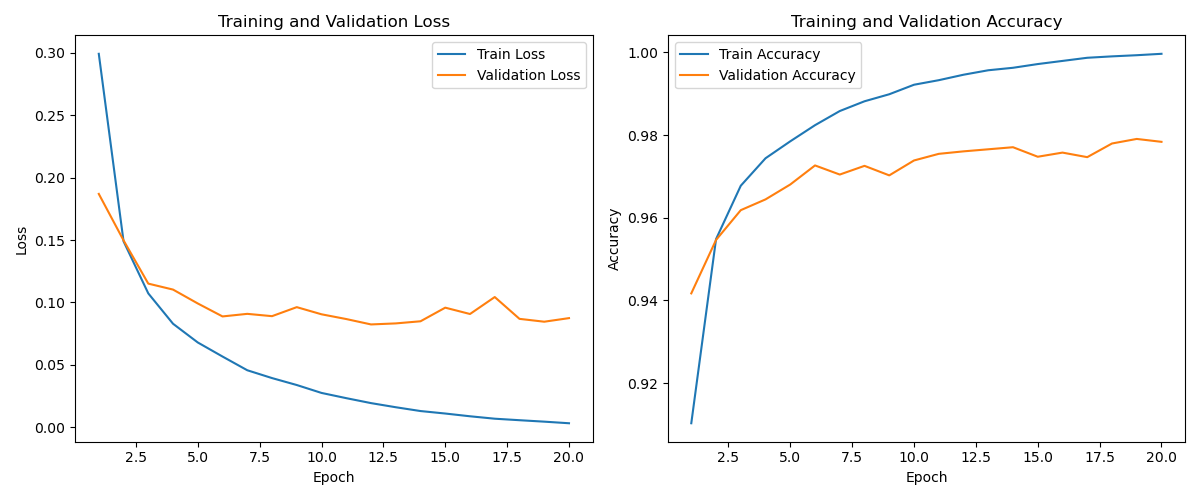
\includegraphics[width=1\linewidth]{Train_Val_Loss_Acc.png} 
     \end{figure}
     \item Test trained network
      \item What is the effect of changing the learning rate:
      \begin{figure}[H]
         \centering
         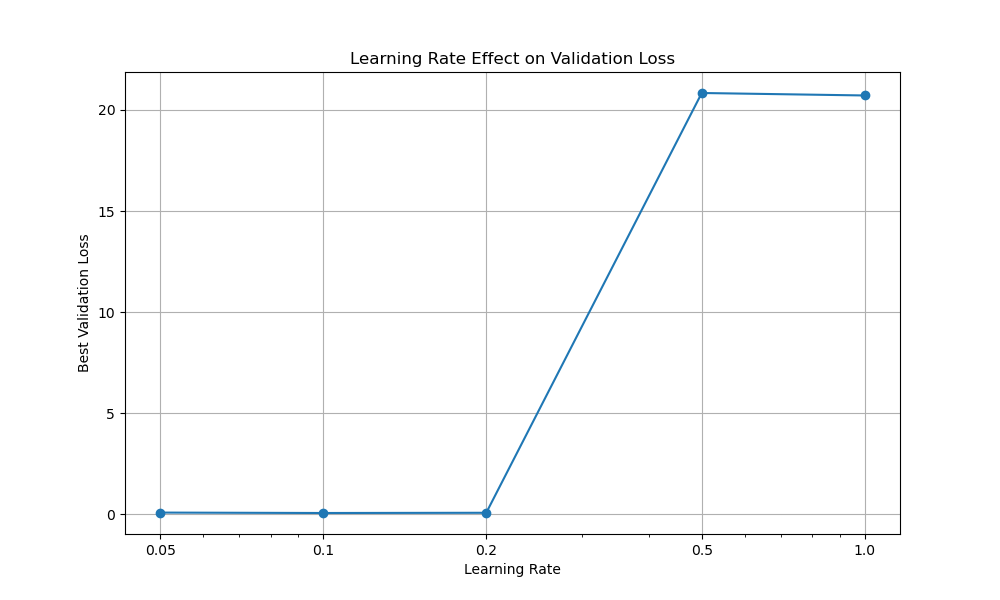
\includegraphics[width=1\linewidth]{lr_comparison.png} 
     \end{figure}
         \begin{itemize}
            \item Too high learning rate leas to the model jumping too far in the weight updates missing the optimal Solutions. The loss also increases instead of decreasing
            \item Too low leearning rate leads to the model to update waits slowly making the training very slow. The training also takes along time to improve
            \item The model convereged to the good solution efficiently on the optimal leanint rate and the training was fast and stable.
         \end{itemize}
   \end{enumerate}

   \subsection*{Bonus Adams}
   How does a properly-tuned Adam Optimizer compare to SGD?
   \begin{itemize}
      \item Adam convergence faster than SGD.
      \item Adam is less sensitive to learning rate than SGD that needs careful tuning
      \item Adam handle noisy gradiesnt well compared to SGD that struggles without momentum
      \item Adam is faster and works well with the minimal tunid however it may not generalize well as a SGD.
      \item SGD with momentum nees more careful tuning but it can lead to better final accuracy in some cases.
   \end{itemize}
   How does the sensitivity of Adam to its learning rate compare to SGD.
   \begin{itemize}
      \item Adam is less sensitive to the initial learning rate than SGD since it adapts to the gradient scale. 
   \end{itemize}

\end{enumerate}


\end{document}